\section{Testing}

Testing agent-based models is difficult because the interaction of agents in a
simulation is dynamic and possibly random which produces complex patterns and
behaviours. Traditional software testing strategies which use the divide and
conquer approach can be applied but will typically miss some undesirable
possibilities due the emergent nature of agent-based systems.

Envisioned possibilities can be easily tested but when a model diverges from
its intended path the relationship between variables could show a bug or even
an unexpected solution. The invariants to a simulation, the relationship of
variables that remain true, can be pre-written or detected during simulation
runs and provide a dynamic way of testing agent-based models.

For example during a simulation run assertions can be placed on variables to
make sure they fall within a certain range. If ranges are not known before hand
they can be detected and the results viewed by the model creator for
correctness.

The testing of individual parts of a system can still achieved by unit testing
but testing the interaction of these parts, integration testing, can use
techniques designed for state machines, and the use of invariant detectors.

\subsection{Unit Testing}

Unit testing is the testing of individual modules of a piece of software, in the
case of models these are the individual agent functions. Each function has an
accompanying unit test function that sets the initial agent memory and any input,
calls the function, and assets that the new agent memory and outputs are of the
expected values.

FLAME provides procedures to help with unit testing:

\begin{itemize}
  \item initialise\_unit\_testing() -- initialises FLAME for unit testing agent
  functions, required at the start of a testing suite.
  \item unittest\_init\_agentname\_agent() -- initialises the agent memory that
  will used in testing
  \item The agent memory is then updated
  \item Messages are sent that will be the input to the function to be tested
  \item The function to be tested is called
  \item Assertions are tested against the resulting agent memory and any output
  \item unittest\_free\_agentname\_agent() -- the agent memory is deleted
  \item free\_messages() -- any messages used are deleted
  \item clean\_up() -- FLAME is finalised and ready to end.
\end{itemize}

Unit testing treats the function to be tested as a black box, inputs are given
and only the outputs are tested, as shown in Figure \ref{fig:unittesting}.

\begin{figure}[hb]
\centering
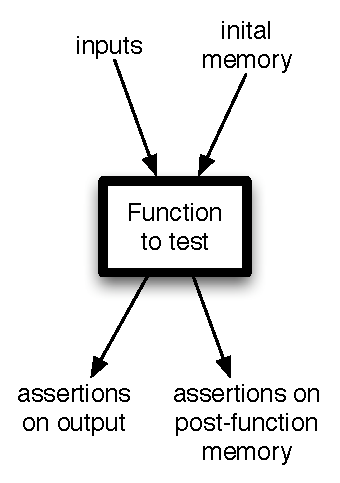
\includegraphics[scale=1.0]{unittest.eps}
\caption{Unit testing}
\label{fig:unittesting}
\end{figure}

\subsection{Integration Testing}


Integration testing is the testing of combinations of individual modules of a
piece of software. Modules that have been unit tested are aggregated into
groups and each group is tested as a whole system. Generating the groups
requires a specific coverage of testing combinations, a test set.

The W-method proposed by T. Chow \cite{CHOW:1978} provides a complete test set
of sequences through a state machine. Because models have been defined as state
machines this technique can be used.

An implementation of the W-method is available through a program called
statechum \cite{WALKINSHAW:2007,WALKINSHAW:2008}
(http://statechum.sourceforge.net/) which accepts as input graphml\\
(http://graphml.graphdrawing.org/), an XML standard for describing graphs.
Each agent as a separate state machine when fed into the W-method will
produce a test set with a specified coverage. An example test set for the Firm
agent in the labour and goods markets is as follows:

{\small
\begin{verbatim}
#1 [Firm_idle, Firm_receive_data, Firm_calc_production_quantity]
#2 [Firm_idle, Firm_idle, Firm_calc_production_quantity, Firm_calc_input_demands, 
    Firm_compute_total_liquidity_needs, Firm_idle, Firm_execute_financial_payments, 
    Firm_calculate_specific_skills_and_wage_offer, Firm_idle, Firm_read_job_quitting,
    Firm_finish_labour_market_first_round, Firm_read_job_quitting_2, Firm_idle,
    Firm_compute_mean_wage_specific_skills, Firm_send_capital_demand,
    Firm_receive_capital_goods, Firm_execute_production, Firm_calc_pay_costs,
    Firm_send_goods_to_mall, Firm_calc_revenue]
#3 [Firm_idle, Firm_idle, Firm_calc_production_quantity, Firm_calc_input_demands,
    Firm_compute_total_liquidity_needs, Firm_idle, Firm_execute_financial_payments,
    Firm_calculate_specific_skills_and_wage_offer, Firm_idle, Firm_read_job_quitting,
    Firm_finish_labour_market_first_round, Firm_read_job_quitting_2,
    Firm_update_wage_offer_2, Firm_compute_mean_wage_specific_skills]
#4 [Firm_idle, Firm_idle, Firm_calc_production_quantity, Firm_calc_input_demands,
    Firm_compute_total_liquidity_needs, Firm_idle, Firm_execute_financial_payments,
    Firm_calculate_specific_skills_and_wage_offer, Firm_idle, Firm_read_job_quitting,
    Firm_start_labour_market, Firm_send_vacancies_2,
    Firm_read_job_applications_send_job_offer_or_rejection_2, Firm_read_job_responses_2,
    Firm_read_job_quitting_2, Firm_idle]
#5 [Firm_idle, Firm_idle, Firm_calc_production_quantity, Firm_calc_input_demands,
    Firm_compute_total_liquidity_needs, Firm_idle, Firm_execute_financial_payments,
    Firm_calculate_specific_skills_and_wage_offer, Firm_send_vacancies,
    Firm_read_job_applications_send_job_offer_or_rejection, Firm_read_job_responses,
    Firm_read_job_quitting, Firm_finish_labour_market_first_round, Firm_read_job_quitting_2,
    Firm_idle]
#6 [Firm_idle, Firm_idle, Firm_calc_production_quantity, Firm_calc_input_demands,
    Firm_compute_total_liquidity_needs, Firm_idle, Firm_execute_financial_payments,
    Firm_calculate_specific_skills_and_wage_offer, Firm_send_vacancies,
    Firm_read_job_applications_send_job_offer_or_rejection, Firm_read_job_responses,
    Firm_read_job_quitting, Firm_update_wage_offer, Firm_send_vacancies_2]
#7 [Firm_idle, Firm_idle, Firm_calc_production_quantity, Firm_calc_input_demands,
    Firm_compute_total_liquidity_needs, Firm_apply_for_loans, Firm_read_loan_acceptance,
    Firm_idle, Firm_execute_financial_payments]
#8 [Firm_idle, Firm_idle, Firm_calc_production_quantity, Firm_calc_input_demands,
    Firm_compute_total_liquidity_needs, Firm_apply_for_loans, Firm_read_loan_acceptance,
    Firm_calc_production_quantity_2, Firm_execute_financial_payments]
#9 [Firm_idle, Firm_idle, Firm_set_quantities_zero, Firm_read_job_quitting,
    Firm_read_job_quitting_2, Firm_calc_revenue, Firm_idle, Firm_send_data_to_Eurostat,
    Firm_send_payments_to_bank]
#10 [Firm_idle, Firm_idle, Firm_set_quantities_zero, Firm_read_job_quitting,
     Firm_read_job_quitting_2, Firm_calc_revenue, Firm_compute_sales_statistics,
     Firm_compute_financial_payments, Firm_compute_income_statement, Firm_compute_dividends,
     Firm_compute_total_financial_payments, Firm_compute_balance_sheet,
     Firm_update_specific_skills_of_workers, Firm_idle]
#11 [Firm_idle, Firm_idle, Firm_set_quantities_zero, Firm_read_job_quitting,
     Firm_read_job_quitting_2, Firm_calc_revenue, Firm_compute_sales_statistics,
     Firm_compute_financial_payments, Firm_compute_income_statement, Firm_compute_dividends,
     Firm_compute_total_financial_payments, Firm_compute_balance_sheet, 
     Firm_update_specific_skills_of_workers, Firm_send_data_to_Eurostat]
#12 [Firm_read_tax_rates, Firm_receive_data]
#13 [Firm_read_tax_rates, Firm_idle]
\end{verbatim}
}

Anticipating the results of individual functions is straight forward. They are
coded for their specific purpose with required results and are therefore easy to
test. With the introduction of communication and interchange of information,
anticipating the results from a group of functions is not so easy, this being
one of the reasons for using agent-based modelling. The consequence of not being
able to predict the results is that first the results have to be created and then
tested for what was roughly expected.

One way to analyse the output of groups of functions is to use an invariant
detector. A program of this type reports any likely invariants, properties that
hold at certain points. This could then be analysed by the modeller and possibly
used as assertions in future test runs.

The Daikon program is an invariant detector \cite{DAIKON:2007}
(http://groups.csail.mit.edu/pag/daikon/). After feeding Daikon the results
from fifty iterations from the labour and goods market model, the invariants
of each agents variables are produced. The examples given below show invariants
of variables where: they keep a certain value; are one of a limited list of
values; or are large or smaller than a certain value. These are only three
types of invariants but Daikon can be told to search for many more, for example
the relationship between two or more variables.

{\small
\begin{verbatim}                        
===========================================================================    
Bank:::OBJECT
id == 1233
region_id == 2
gov_id == 1232
last_credit_id == 0
amount_credit_offer == 0.0
total_deposits one of { 0.0, 1808.8 }
total_loan_supply one of { 0.0, 1627.92 }
===========================================================================
Eurostat:::OBJECT
id == 1236
region_id == 2
num_households == 0
unemployment_rate == 0.0
average_s_skill == 1.0
no_firms == 0
gdp == 0.0
===========================================================================
Firm:::OBJECT
id >= 1
region_id one of { 1, 2 }
gov_id == 1232
day_of_month_to_act == 0
payment_account == 50.0
wage_offer == 1.0
average_g_skill == 0.0
ebit == 0.0
tax_rate_corporate == 0.25
earnings_per_share == 0.01
current_shares_outstanding == 1200
total_value_capital_stock == 200.0
planned_value_capital_stock == 2.0
bank_id == 1233
mean_specific_skills == 0.8
out_of_stock_costs one of { 0.0, 1.0 }
===========================================================================
Government:::OBJECT
id == 1232
bank_id == 1233
payment_account == 100.0
tax_revenues == 0.0
unemployment_benefit_payment == 0.8
tax_rate_corporate == 0.25
num_unemployed == 0
===========================================================================
Household:::OBJECT
region_id one of { 1, 2 }
gov_id == 1232
bank_id == 1233
day_of_month_to_act == 0
payment_account == 0.8
wage == 0.0
wage_reservation == 1.0
general_skill >= 1
number_applications == 15
last_labour_income == 0.0
employee_firm_id == -1
employer_region_id == 0
week_of_month one of { 3, 4 }
mall_completely_sold_out one of { 0, 1 }
day_of_week_to_act >= 0
tax_rate_hh_capital == 0.25
===========================================================================
IGFirm:::OBJECT
id == 31
region_id == 2
gov_id == 1232
bank_id == 1233
day_of_month_to_act == 0
payment_account == 0.0
productivity == 1.0
capital_good_price == 100.0
tax_rate_corporate == 0.25
tax_payment == 0.0
outstanding_shares == 1200
===========================================================================
Mall:::OBJECT
id one of { 1234, 1235 }
region_id one of { 1, 2 }
gov_id == 0
total_supply == 0.0
\end{verbatim}
}

This technique can be utilised for tracking changes of variables between
functions and not just between iterations giving more testing coverage of
groups of functions.
